\chapter{Experimental Results}

% At some point you will have to determine whether your project works. This
% section should detail the design of the testing experiments, the results of
% the testing, and comments regarding whether the project does what it is
% supposed to do.  Elements that are hard to test and aspects of the project
% that do not pass the tests should be highlighted.  The design of the
% experiments is worth some space as well, as there are design tradeoffs and
% decisions to be discussed here as well as for the project itself.  Any data
% should be included in tables or charts in this section or in an appendix if
% it is particularly cumbersome.

\section{Introduction}

How well the HUD system works overall is a qualitative judgement. We decided the system
was complete when we could drive around with it.
However, we did have some requirements on performance for the power suppy unit, as well
as for the OBD subsystem.

\section{Power Supply Unit}

The main requirement for the power supply was that it needed to handle transient 
situations and protect the rest of the system.  The power supply was able to survive
cold-cranking which sees input voltages as low as 4.5V.  It was also tested
over its entire supply range (3.5 to 18 volts) and worked over all voltages.  The PSU
also shutdown as designed when the input voltage was outside of this range.  The 
testing of severe transient conditions ($\pm 100$V) requires special equipment that was
not available to us and thus we were able to completely verify protection in these
situations.

While not a requirement of the project, a high-efficiency power supply is advantageous 
due to decreased power draw and heat generation.  With approximately 60\% loads on 
each rail, the entire board is close to 90\% efficient.  This was achieved with a 
careful PCB layout and efficient switching regulator ICs.

\section{On-Board Diagnostics Interface}

The refresh rate of vehicle data on the display is our core measurement of
performance for this subsystem. Overall, it seems that we can request a value
from the vehicle and place it on the display in around 100 milliseconds. This
is fast enough to seem as responsive as the vehicle's needles. Response times
vary depending on the internal protocol of the vehicle's electronics system, but
qualitatively the difference was not severe.

\section{Overall System Usability}

The system functons well overall. The VFD was very bright and clear, and only
in direct sunlight was it at all difficult to see. Figure~\ref{fig:display-day}
shows the display during the day, and figure~\ref{fig:display-night} shows
the display at night.  The aberrations created by the imperfect mirror can 
easil be seen at night.

\begin{figure}[h]
\includegraphics[width=\textwidth]{img/display_day.png}
\caption{The display during the day}
\label{fig:display-day}
\end{figure}

\begin{figure}[h]
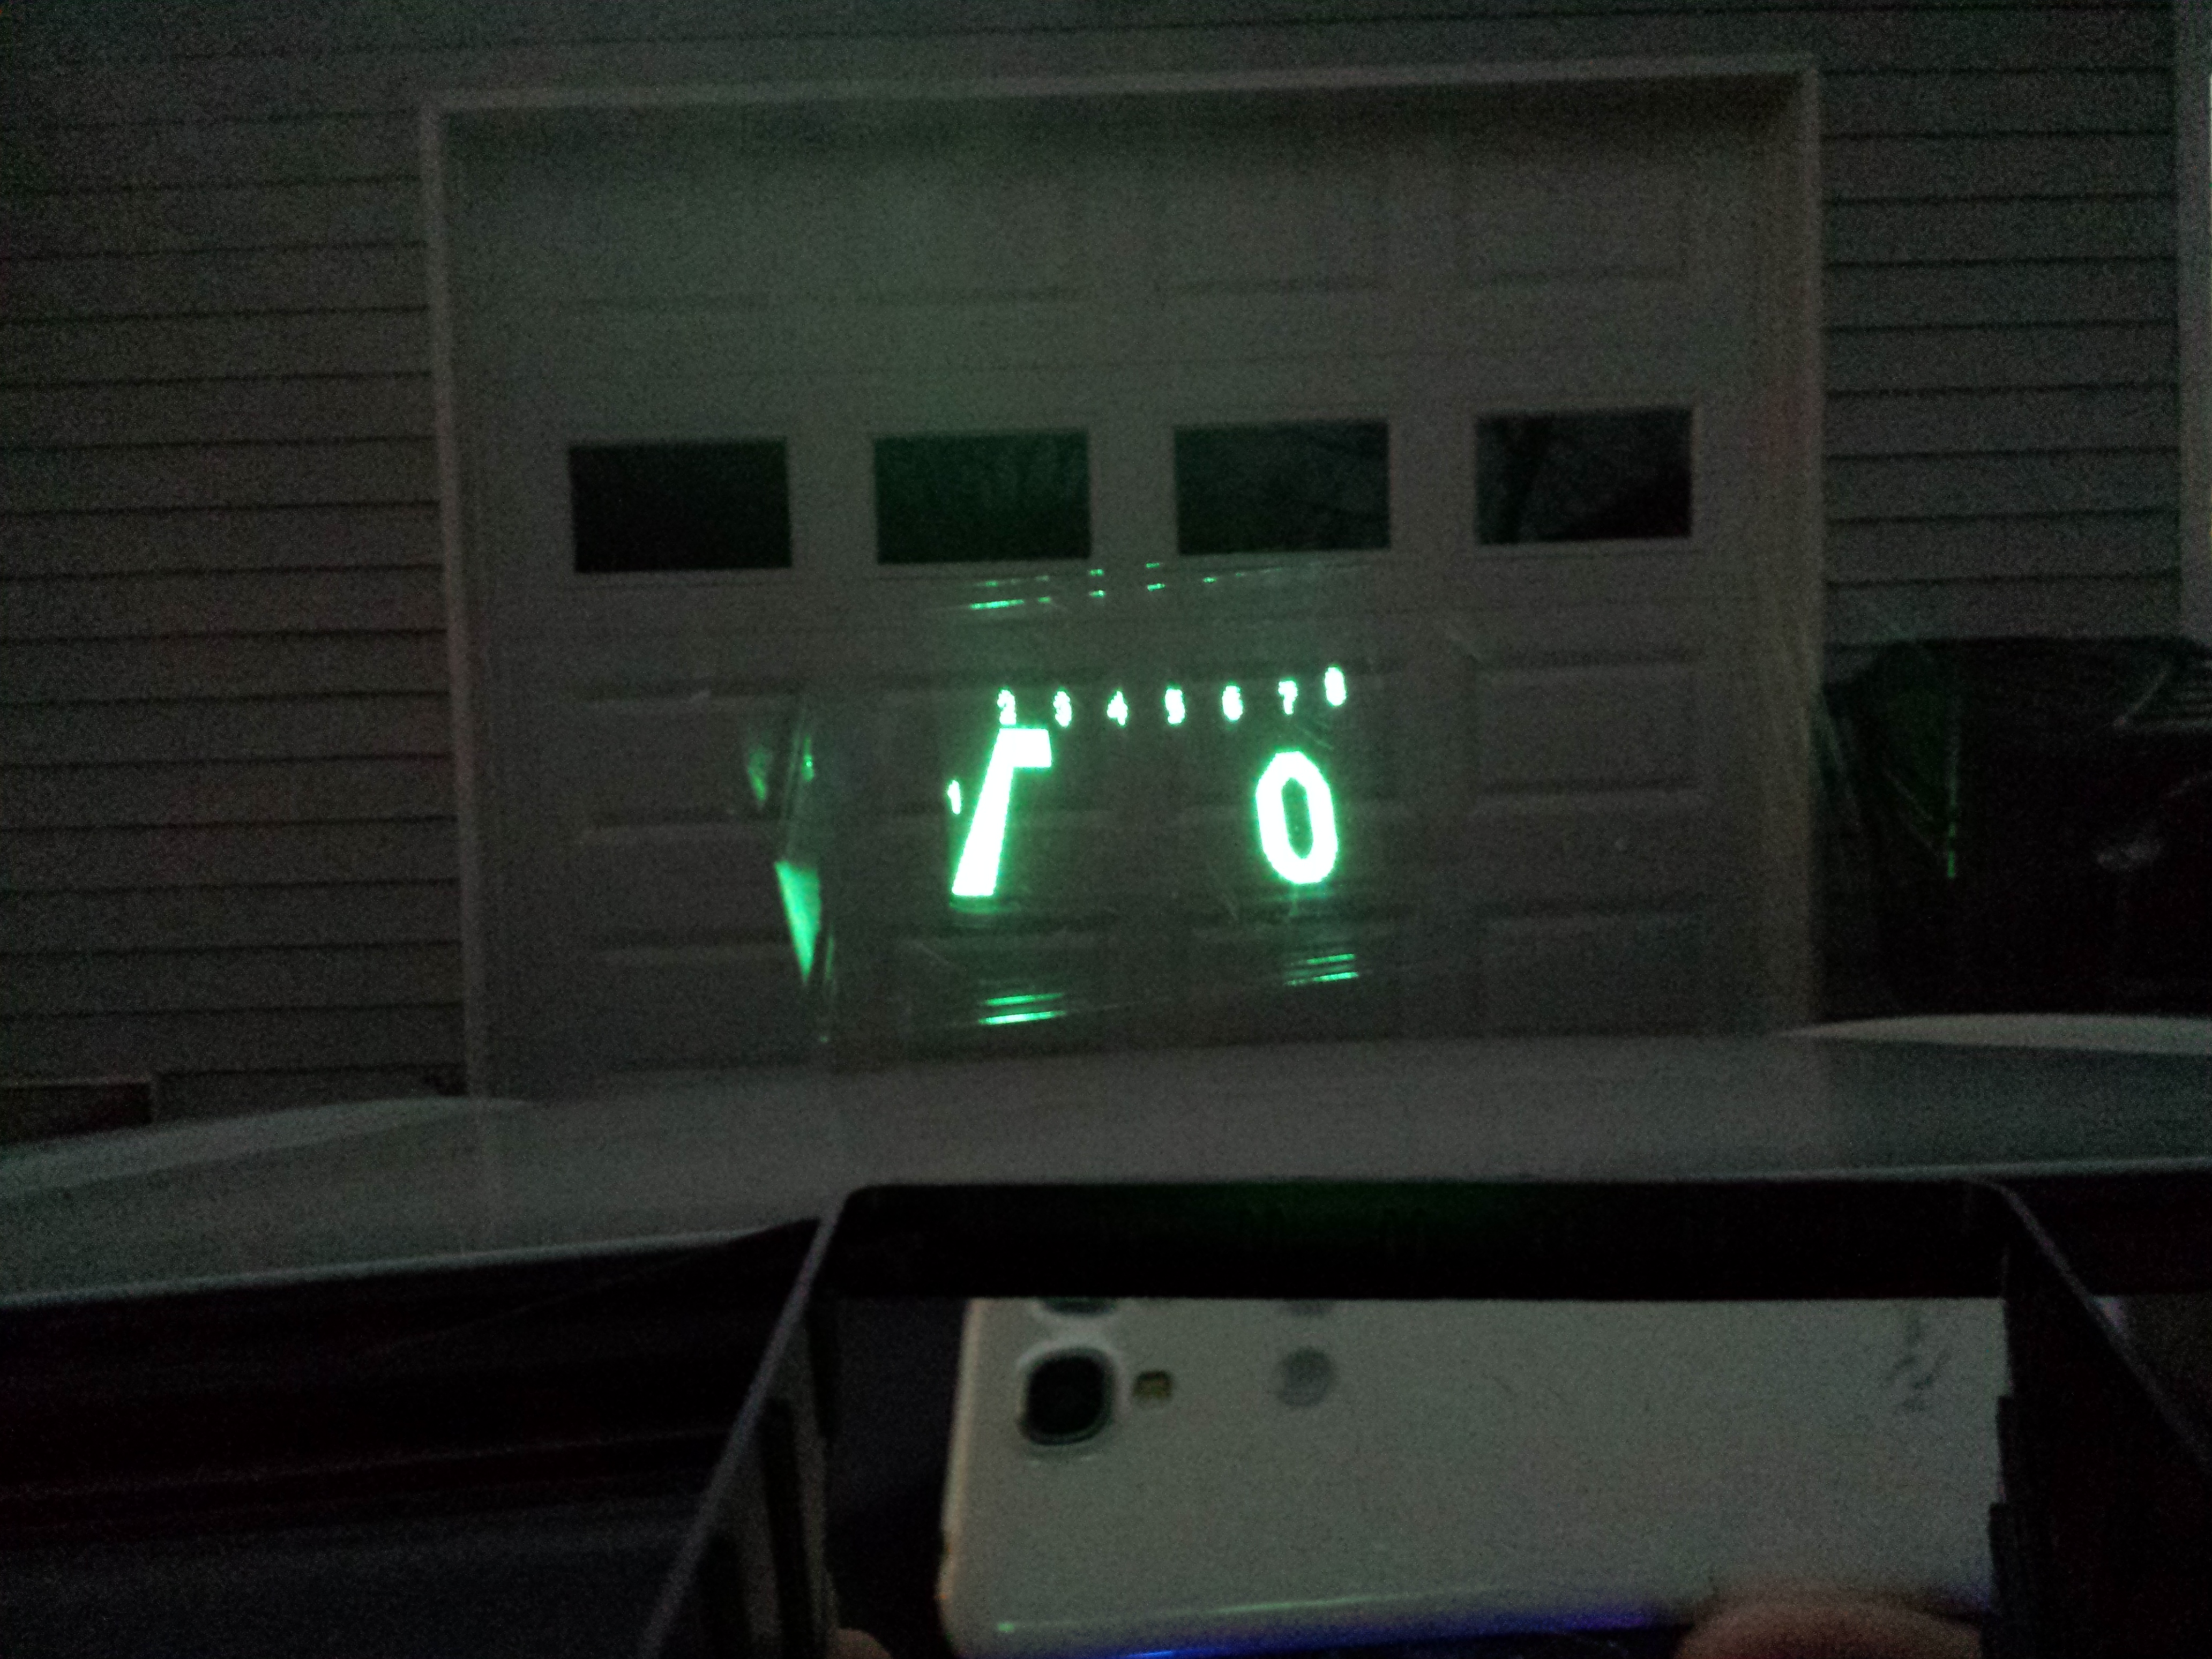
\includegraphics[width=\textwidth]{img/display_night.jpg}
\caption{The display at night}
\label{fig:display-night}
\end{figure}

Some videos of the functional system can be found on Youtube:

\begin{description}
\item[VFD only]\url{http://youtu.be/Lh0EtPrTeFc}
\item[Road test] \url{http://youtu.be/hr66TgOQNoI}
\end{description}
